% ctex_test.tex
\documentclass[UTF8]{ctexart}
\usepackage{setspace}
\usepackage[letterpaper,top=2cm,bottom=2cm,left=3cm,right=3cm,marginparwidth=1.75cm]{geometry}
\usepackage{listings}
\usepackage{xcolor}      %代码着色宏包
\usepackage{amsmath}
\usepackage{mathabx}
\usepackage{tikz}
\usepackage{verbatim}
\usepackage{graphicx}
\CTEXsetup[format={\Large\bfseries}]{section}

\title{Numerical Analysis Project2}
\author{数学与应用数学2002 王锦宸 }
\date{October 2022}

\begin{document}

\maketitle

\section*{B}
\noindent when n = 2,\\
the polynomial is:\\$0.03846+0.19231(x+5)-0.03846(x+5)x$\\
when n = 4,\\
the polynomial is:\\$0.03846+0.03979(x+5)+0.06101(x+5)(x+2.5)-0.02653(x+5)(x+2.5)x+0.00531(x+5)(x+2.5)x(x-2.5)$\\
when n = 6,\\
the polynomial is:\\$0.03846+0.02646(x+5)+0.02485(x+5)(x+3.33333)+0.01494(x+5)(x+3.33333)(x+1.66667)-0.01317(x+5)(x+3.33333)(x+1.66667)x+0.00420(x+5)(x+3.33333)(x+1.66667)x(x-1.66667)-0.00084(x+5)(x+3.33333)(x+1.66667)x(x-1.66667)(x-3.33333)$\\
when n = 8,\\
the polynomial is:\\$0.03846+0.02234(x+5)+0.01396(x+5)(x+3.75)+0.01170(x+5)(x+3.75)(x+2.5)+0.00067(x+5)(x+3.75)(x+2.5)(x+1.25)-0.00490(x+5)(x+3.75)(x+2.5)(x+1.25)x+0.00244(x+5)(x+3.75)(x+2.5)(x+1.25)x(x-1.25)-0.00069(x+5)(x+3.75)(x+2.5)(x+1.25)x(x-1.25)(x-2.5)+0.00014(x+5)(x+3.75)(x+2.5)(x+1.25)x(x-1.25)(x-2.5)(x-3.75)$\\
\\
The plot is drawn by \textbf{\textit{GEOGEBRA}} as follows.
\graphicspath{{Images/}}
\begin{figure}[htp]
    \centering
    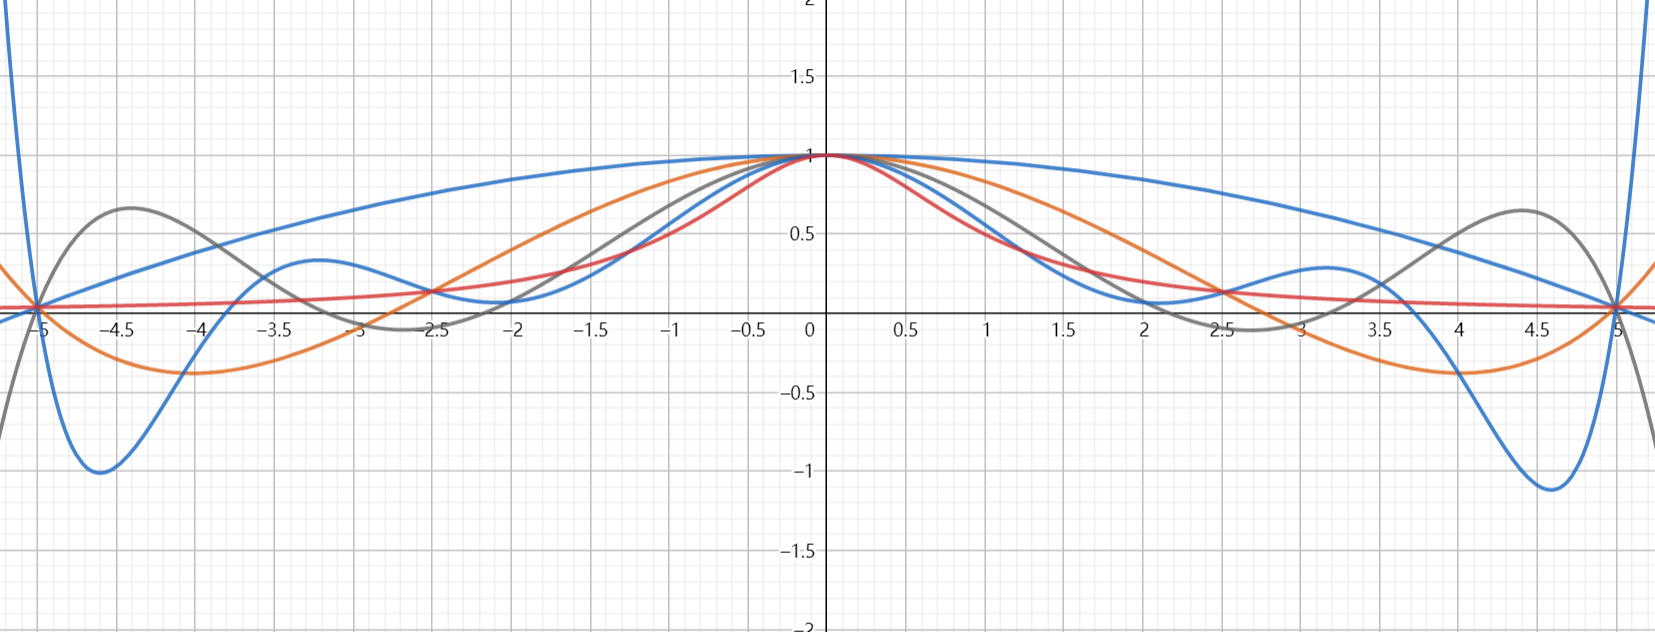
\includegraphics[width=10cm]{PlotB}
    \caption{The Plot of Runge phenomenon}
    \label{fig:PlotB}
\end{figure}

\section*{C}
\noindent Since the polynomial is too long, we only display the plot.
In this Problem, we choose the interpolating points to be the zeros of Chebyshev polynomials Tn,
$$x_k = cos\left(\frac{2k-1}{2n}\right) \qquad k = 1,\dots,n$$
The plot is displayed as follows.\\
\begin{figure}[htp]
    \centering
    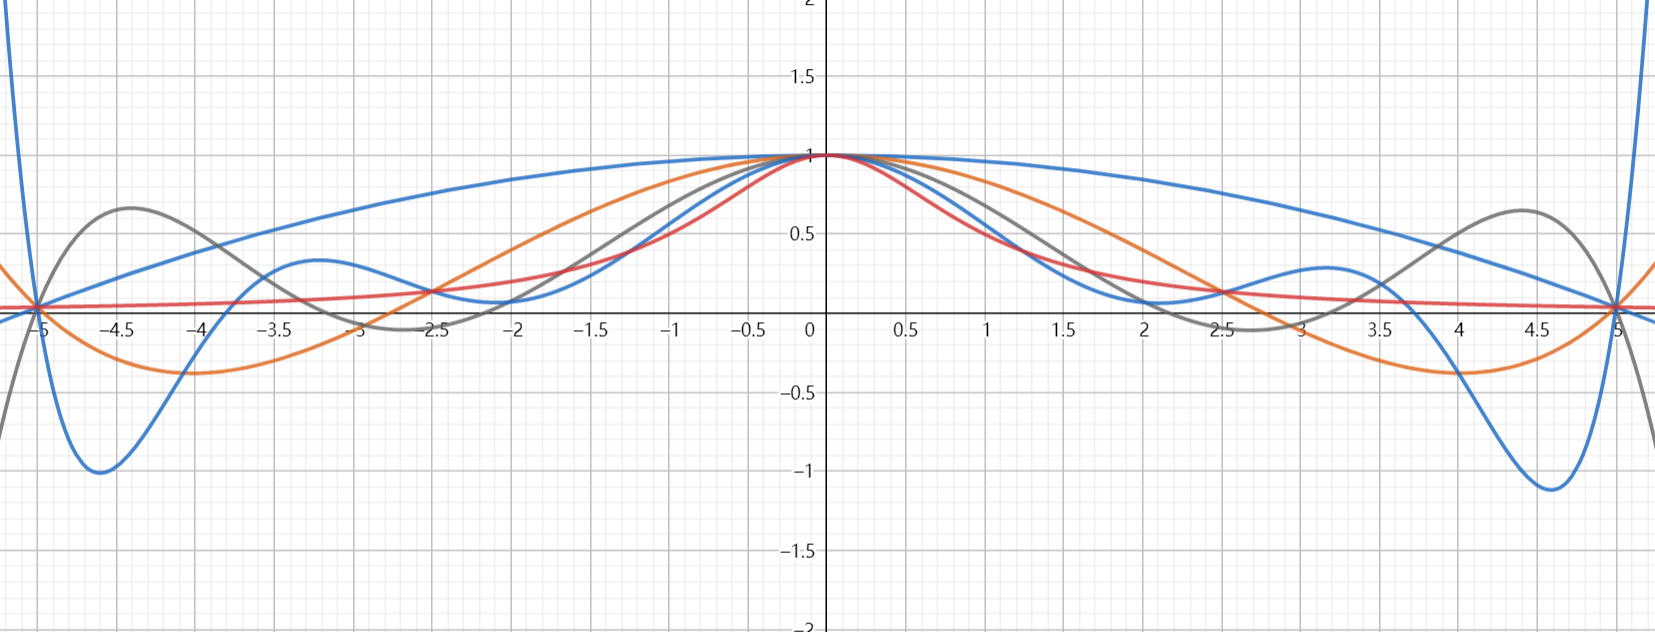
\includegraphics[width=10cm]{PlotB}
    \caption{The Plot of Runge phenomenon}
    \label{fig:PlotC}
\end{figure}

\section*{D}
\noindent 
(a) f(10) = 742.5 and f'(10) = 48.38\\
(b) As is displayed in the plot below, we can easily find that car has exceeded the speed limit.\\
\begin{figure}[htp]
    \centering
    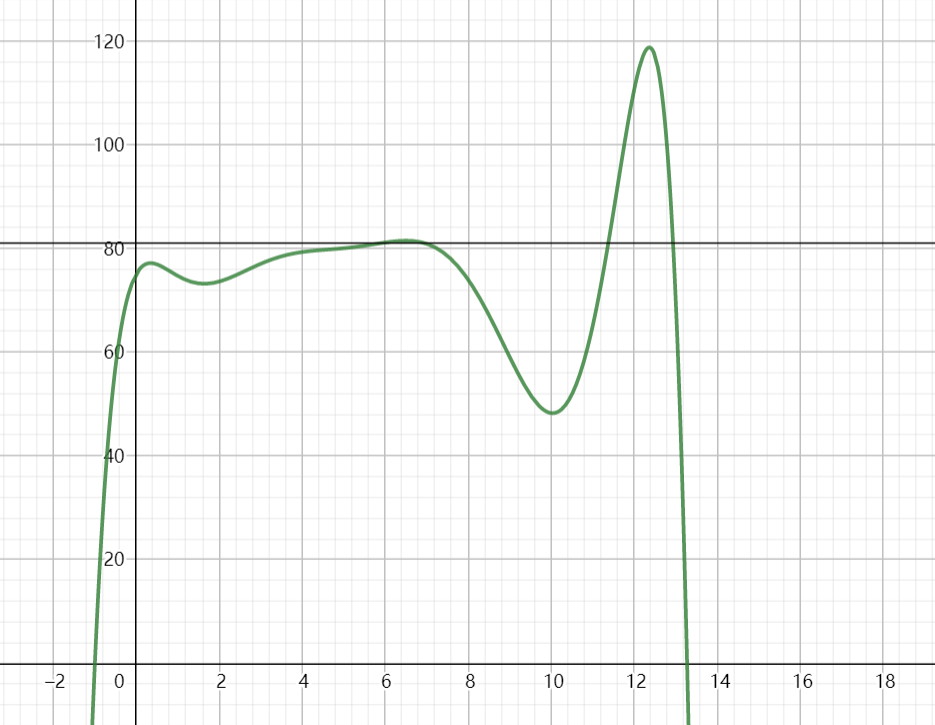
\includegraphics[width=10cm]{PlotD}
    \caption{Speed Curve}
    \label{fig:PlotD}
\end{figure}

\section*{E}
(a)$p_1(x) = 6.67+1.77167*x+0.45783*x(x-6)-0.12478*x(x-6)(x-10)+0.01357*x(x-6)(x-10)(x-13)-0.00098*x(x-6)(x-10)(x-13)(x-17)+0.00004*x(x-6)(x-10)(x-13)(x-17)(x-20)$\\
$p_2(x) = 6.67+1.57167*x-0.08717*x(x-6)-0.01527*x(x-6)(x-10)+0.00258*x(x-6)(x-10)(x-13)-0.00020*x(x-6)(x-10)(x-13)(x-17)+0.00001*x(x-6)(x-10)(x-13)(x-17)(x-20)$\\
(b)According to the plot as follows, the larvae will be still alive in day43 and will even be immortal.
\begin{figure}[htp]
    \centering
    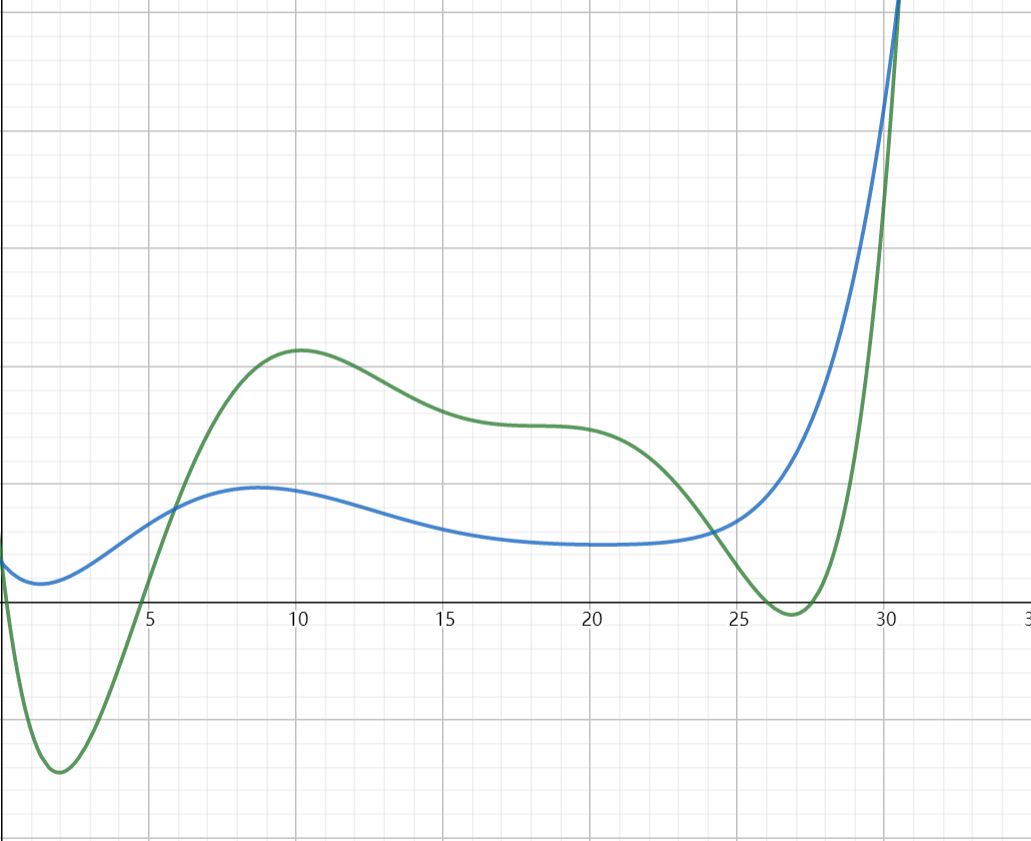
\includegraphics[width=10cm]{PlotE}
    \caption{Larvae Curve}
    \label{fig:PlotE}
\end{figure}
\end{document}

